\section{Sample System Ouput - Units Data}
This section contains data that has been converted from it's raw sensor readings to calibrated readings with units.
\begin{figure}[]
	\centering
	\caption{accelX vs. Time}
		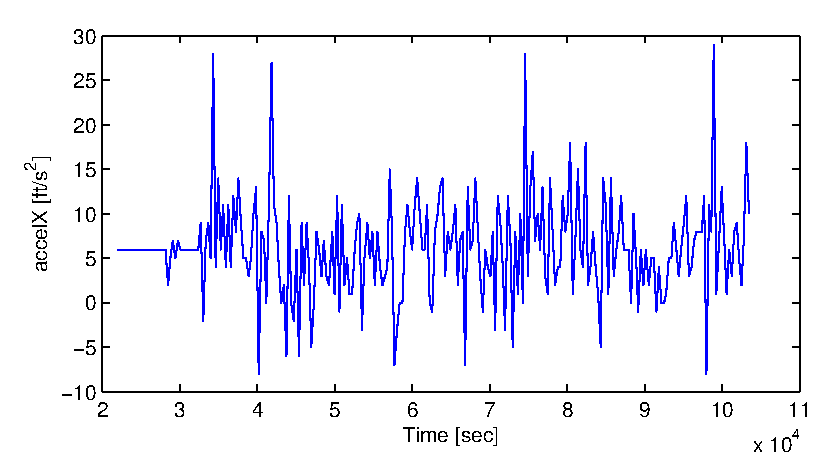
\includegraphics[width = 0.7\textwidth]{C:/Users/mufasa/Documents/Thesis/LaTex/figures/sampleOutput/Units/accelX.eps}
\end{figure}
\begin{figure}[]
	\centering
	\caption{accelY vs. Time}
		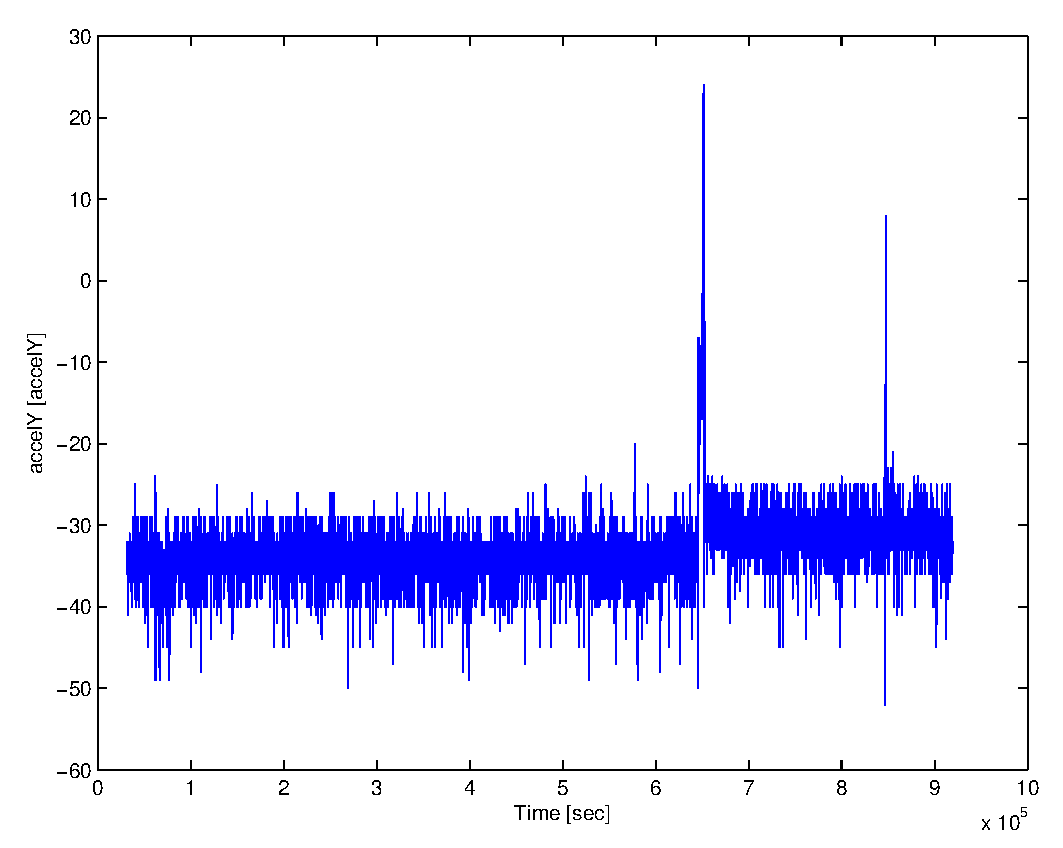
\includegraphics[width = 0.7\textwidth]{C:/Users/mufasa/Documents/Thesis/LaTex/figures/sampleOutput/Units/accelY.eps}
\end{figure}
\begin{figure}[]
	\centering
	\caption{accelZ vs. Time}
		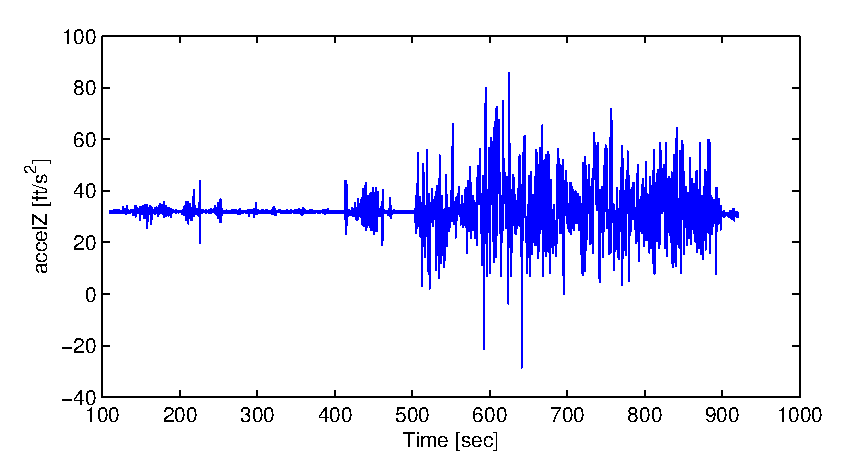
\includegraphics[width = 0.7\textwidth]{C:/Users/mufasa/Documents/Thesis/LaTex/figures/sampleOutput/Units/accelZ.eps}
\end{figure}
\begin{figure}[]
	\centering
	\caption{gyroX vs. Time}
		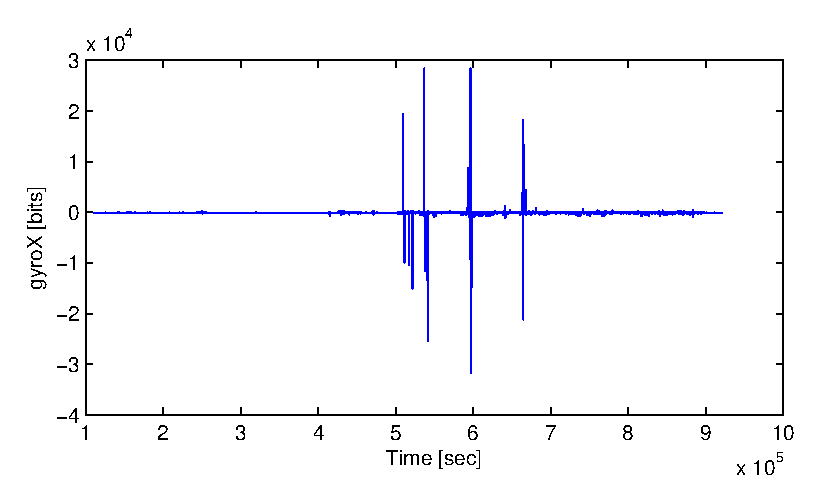
\includegraphics[width = 0.7\textwidth]{C:/Users/mufasa/Documents/Thesis/LaTex/figures/sampleOutput/Units/gyroX.eps}
\end{figure}
\begin{figure}[]
	\centering
	\caption{gyroY vs. Time}
		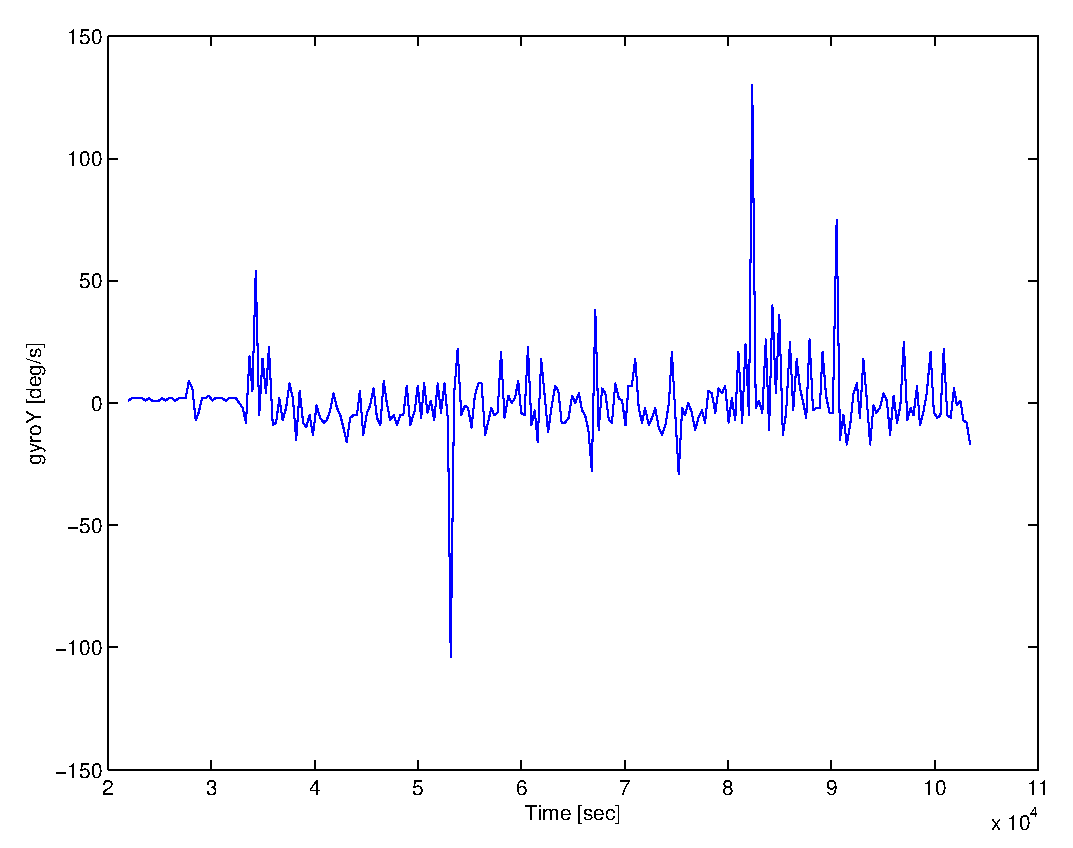
\includegraphics[width = 0.7\textwidth]{C:/Users/mufasa/Documents/Thesis/LaTex/figures/sampleOutput/Units/gyroY.eps}
\end{figure}
\begin{figure}[]
	\centering
	\caption{gyroZ vs. Time}
		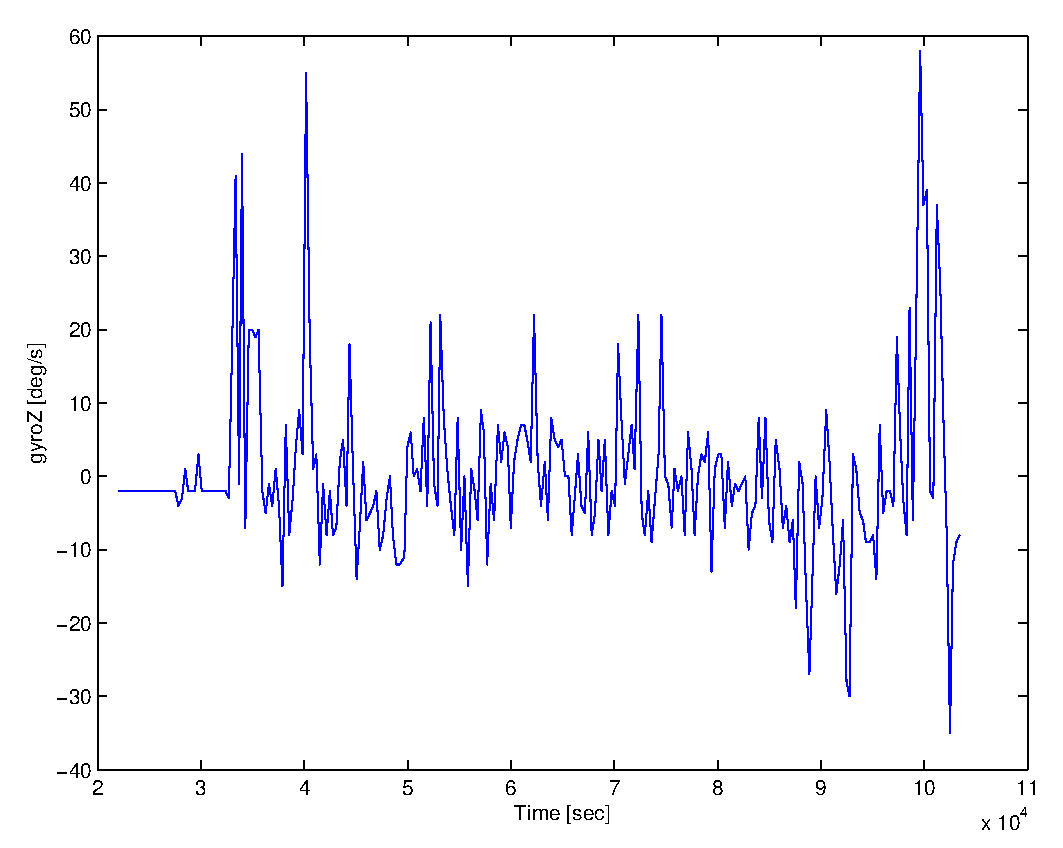
\includegraphics[width = 0.7\textwidth]{C:/Users/mufasa/Documents/Thesis/LaTex/figures/sampleOutput/Units/gyroZ.eps}
\end{figure}
\clearpage
\begin{figure}[]
	\centering
	\caption{magX vs. Time}
		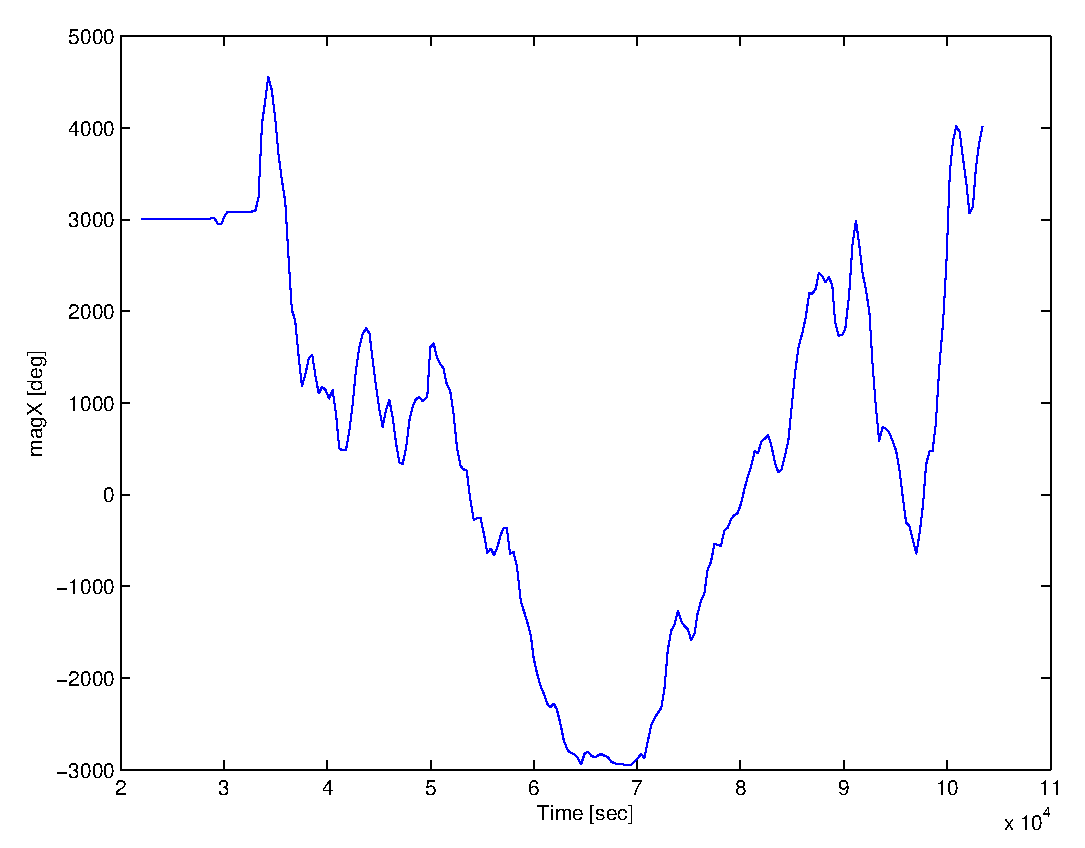
\includegraphics[width = 0.7\textwidth]{C:/Users/mufasa/Documents/Thesis/LaTex/figures/sampleOutput/Units/magX.eps}
\end{figure}
\begin{figure}[]
	\centering
	\caption{magY vs. Time}
		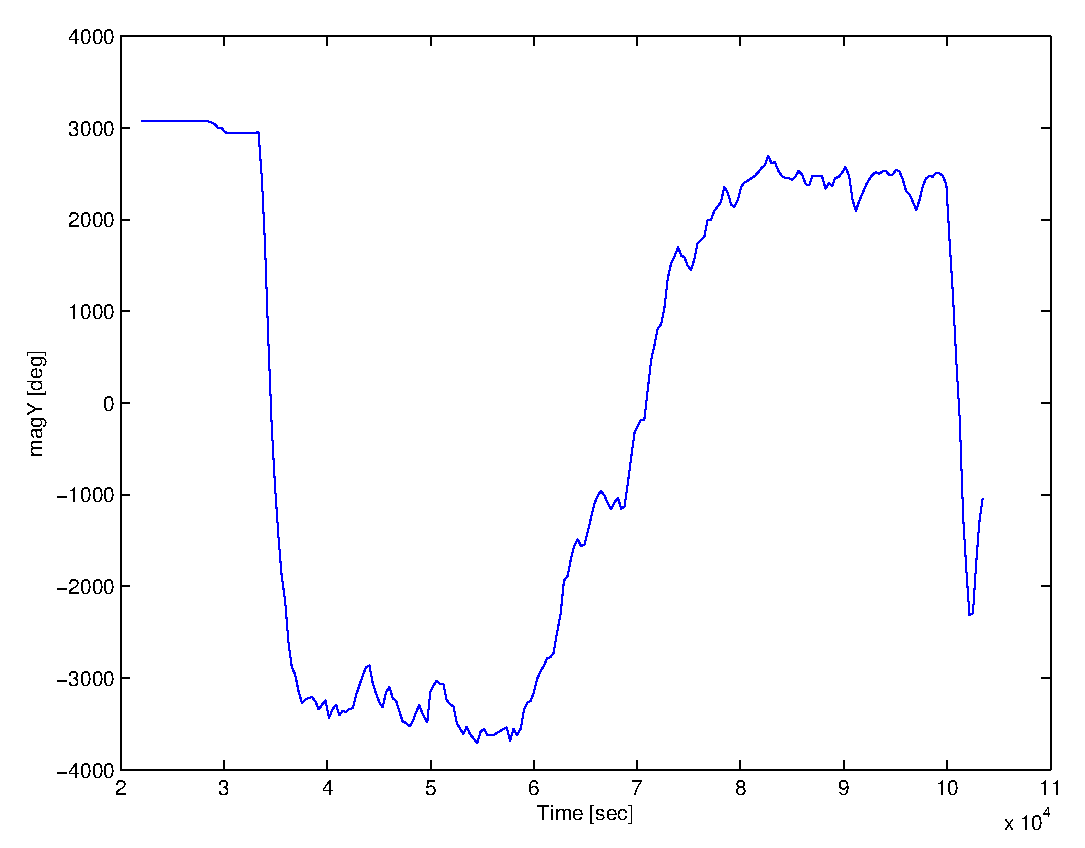
\includegraphics[width = 0.7\textwidth]{C:/Users/mufasa/Documents/Thesis/LaTex/figures/sampleOutput/Units/magY.eps}
\end{figure}
\begin{figure}[]
	\centering
	\caption{magZ vs. Time}
		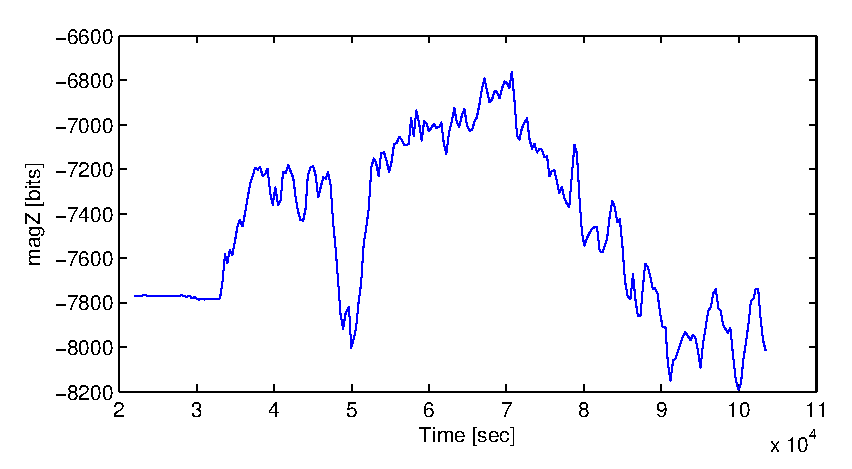
\includegraphics[width = 0.7\textwidth]{C:/Users/mufasa/Documents/Thesis/LaTex/figures/sampleOutput/Units/magZ.eps}
\end{figure}
\begin{figure}[]
	\centering
	\caption{press0 vs. Time}
		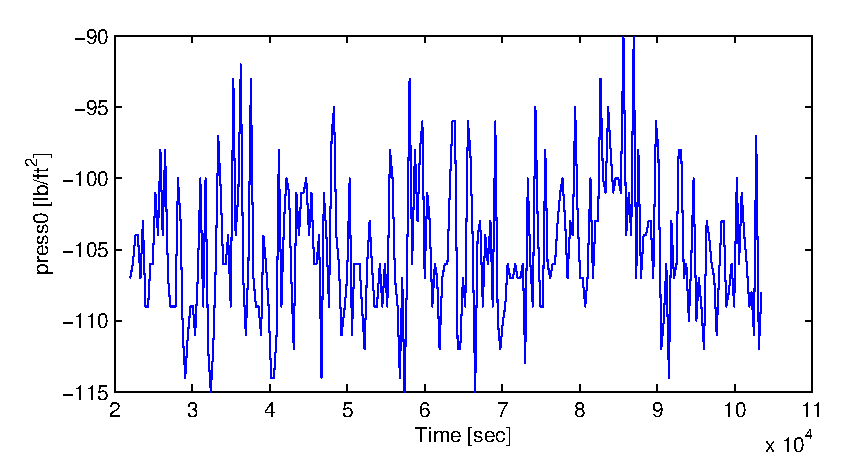
\includegraphics[width = 0.7\textwidth]{C:/Users/mufasa/Documents/Thesis/LaTex/figures/sampleOutput/Units/press0.eps}
\end{figure}
\begin{figure}[]
	\centering
	\caption{press1 vs. Time}
		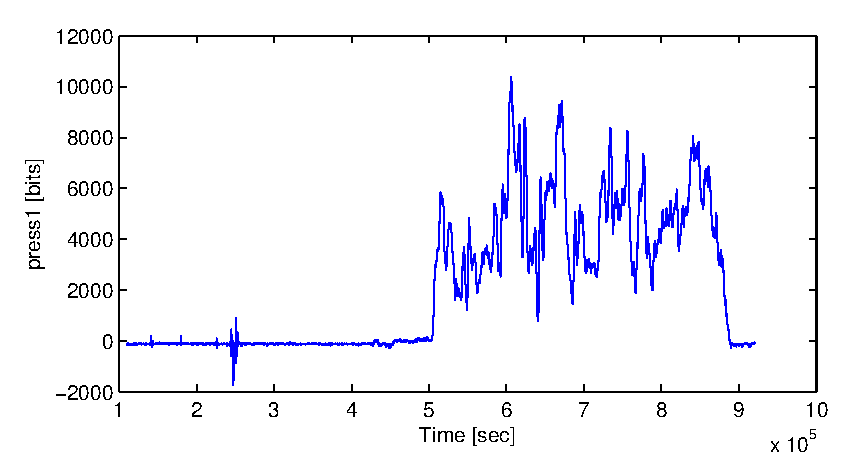
\includegraphics[width = 0.7\textwidth]{C:/Users/mufasa/Documents/Thesis/LaTex/figures/sampleOutput/Units/press1.eps}
\end{figure}
\begin{figure}[]
	\centering
	\caption{press2 vs. Time}
		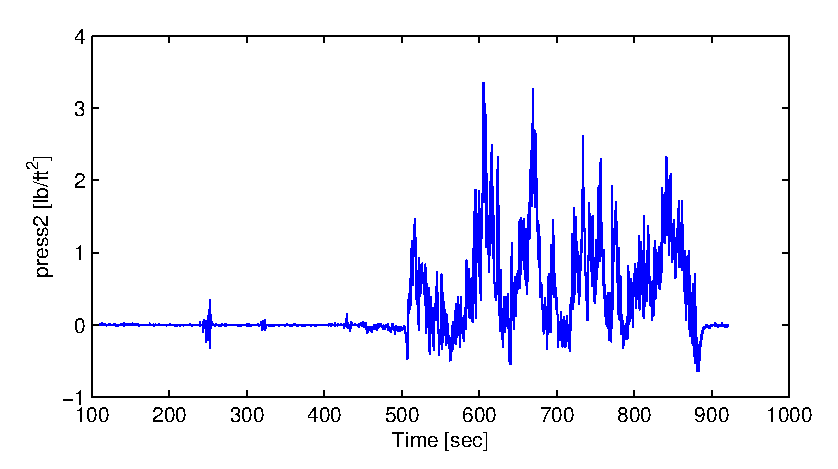
\includegraphics[width = 0.7\textwidth]{C:/Users/mufasa/Documents/Thesis/LaTex/figures/sampleOutput/Units/press2.eps}
\end{figure}
\begin{figure}[]
	\centering
	\caption{press3 vs. Time}
		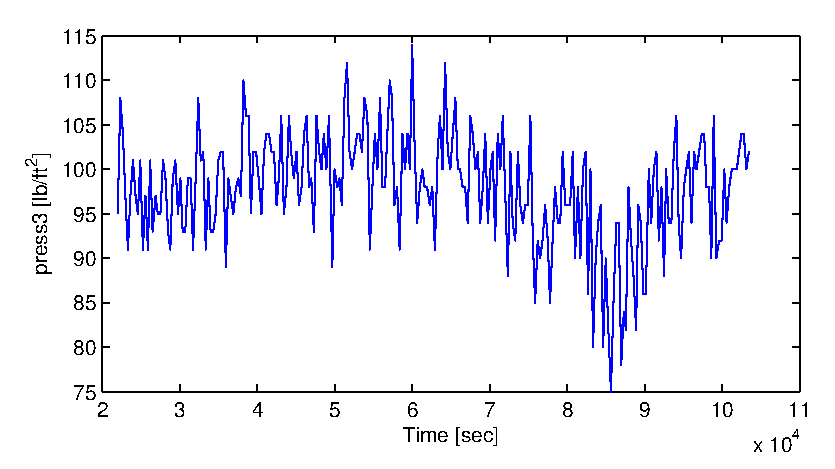
\includegraphics[width = 0.7\textwidth]{C:/Users/mufasa/Documents/Thesis/LaTex/figures/sampleOutput/Units/press3.eps}
\end{figure}
\begin{figure}[]
	\centering
	\caption{gpsLat vs. Time}
		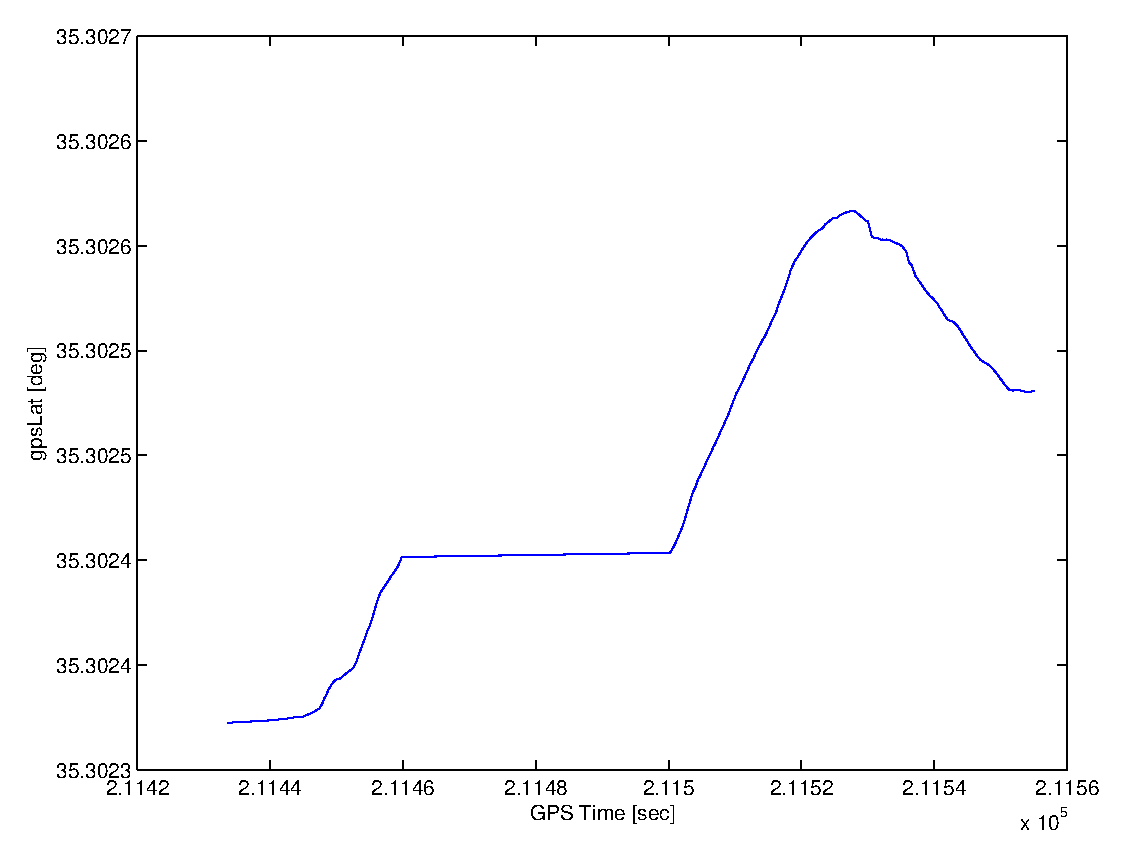
\includegraphics[width = 0.7\textwidth]{C:/Users/mufasa/Documents/Thesis/LaTex/figures/sampleOutput/Units/gpsLat.eps}
\end{figure}
\begin{figure}[]
	\centering
	\caption{gpsLong vs. Time}
		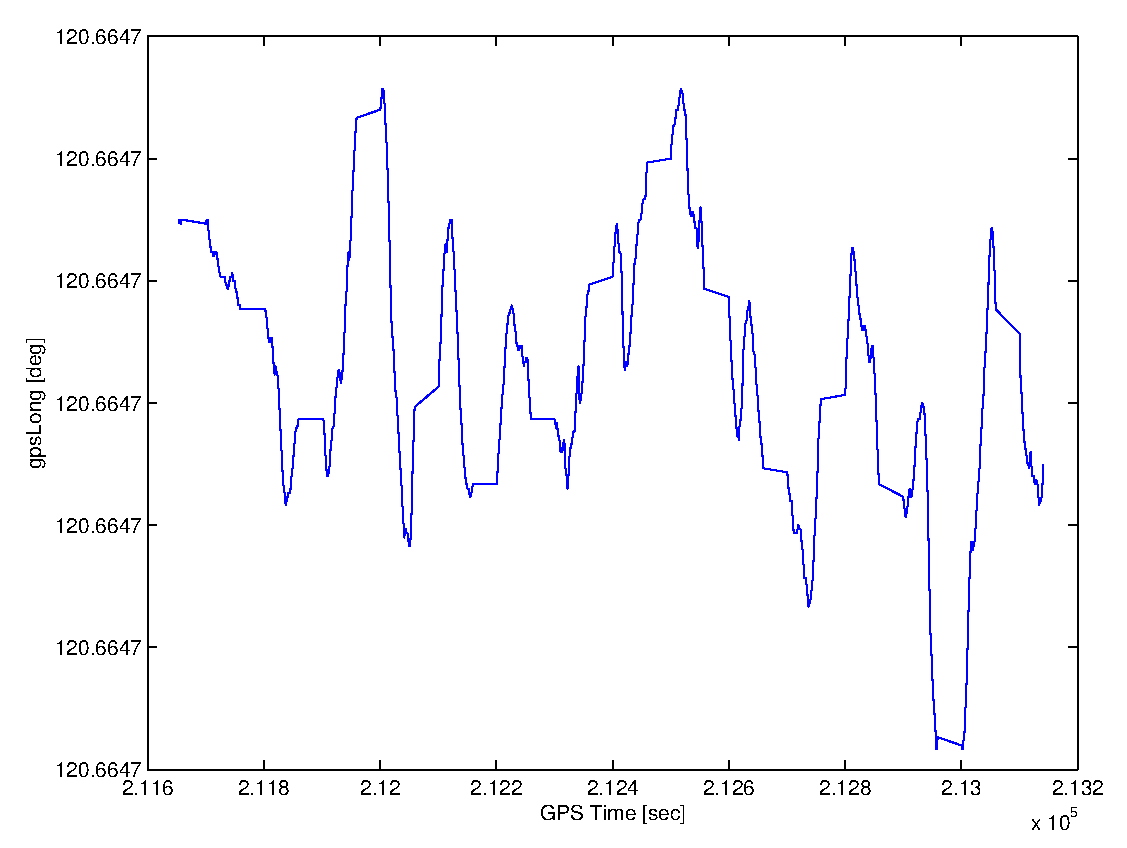
\includegraphics[width = 0.7\textwidth]{C:/Users/mufasa/Documents/Thesis/LaTex/figures/sampleOutput/Units/gpsLong.eps}
\end{figure}
\begin{figure}[]
	\centering
	\caption{gpsSpd vs. Time}
		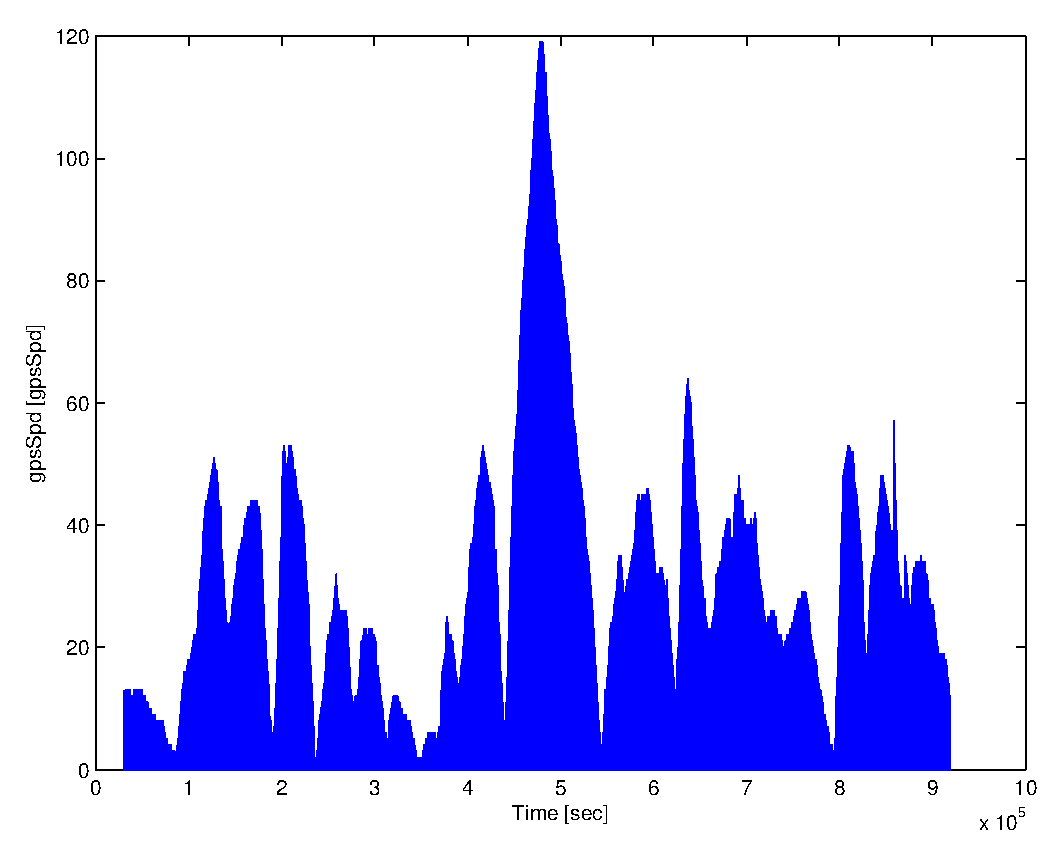
\includegraphics[width = 0.7\textwidth]{C:/Users/mufasa/Documents/Thesis/LaTex/figures/sampleOutput/Units/gpsSpd.eps}
\end{figure}
\begin{figure}[]
	\centering
	\caption{gpsCrs vs. Time}
		\includegraphics[width = 0.7\textwidth]{C:/Users/mufasa/Documents/Thesis/LaTex/figures/sampleOutput/Units/gpsCrs.eps}
\end{figure}
\begin{figure}[]
	\centering
	\caption{date vs. Time}
		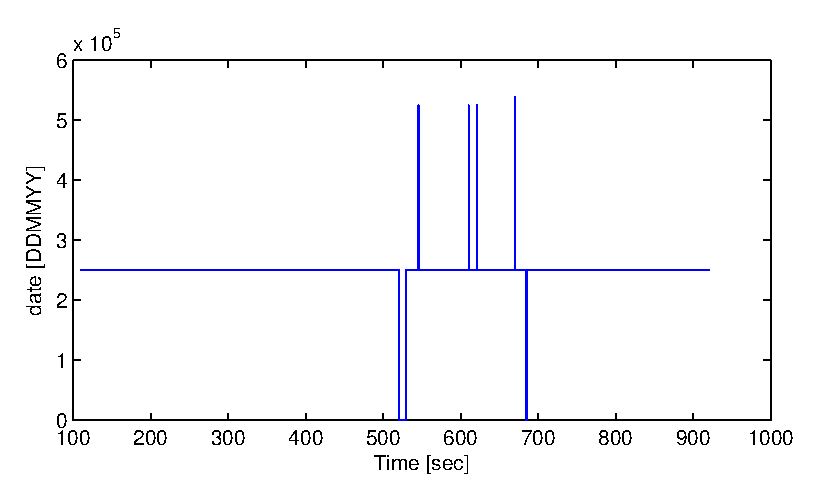
\includegraphics[width = 0.7\textwidth]{C:/Users/mufasa/Documents/Thesis/LaTex/figures/sampleOutput/Units/date.eps}
\end{figure}
\begin{figure}[]
	\centering
	\caption{CS vs. Time}
		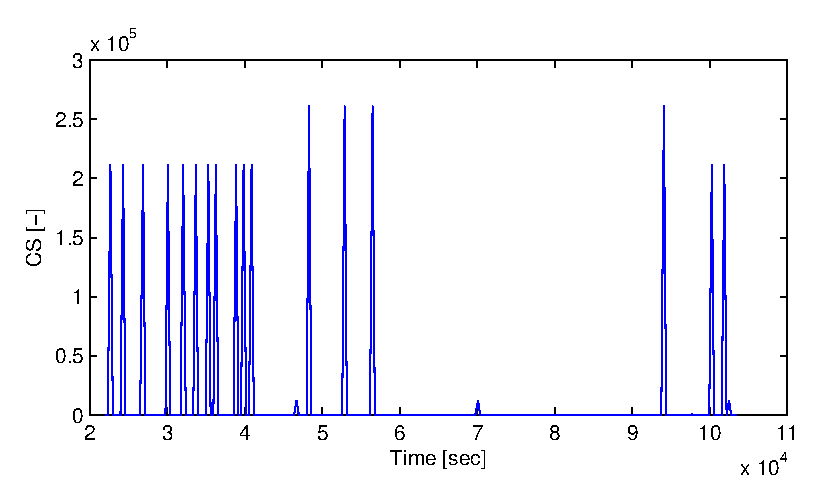
\includegraphics[width = 0.7\textwidth]{C:/Users/mufasa/Documents/Thesis/LaTex/figures/sampleOutput/Units/CS.eps}
\end{figure}
\begin{figure}[]
	\centering
	\caption{temperature vs. Time}
		\includegraphics[width = 0.7\textwidth]{C:/Users/mufasa/Documents/Thesis/LaTex/figures/sampleOutput/Units/temperature.eps}
\end{figure}
\begin{figure}[]
	\centering
	\caption{deltaT vs. Time}
		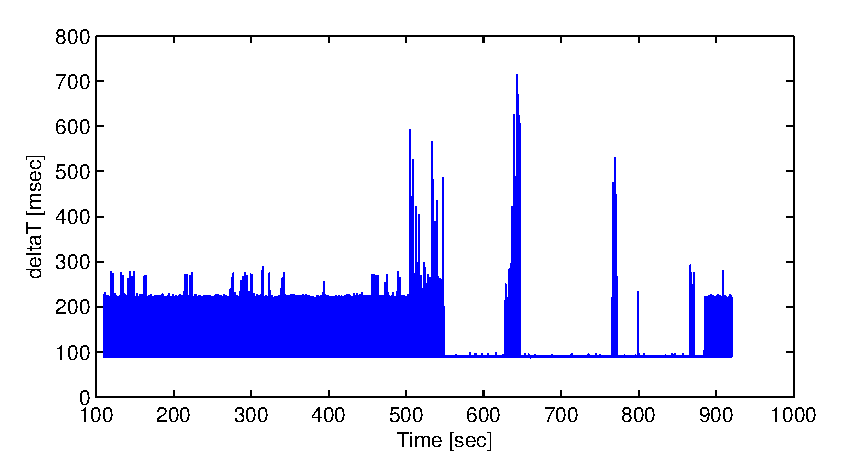
\includegraphics[width = 0.7\textwidth]{C:/Users/mufasa/Documents/Thesis/LaTex/figures/sampleOutput/Units/deltaT.eps}
\end{figure}
\begin{figure}[]
	\centering
	\caption{rpmPwm vs. Time}
		\includegraphics[width = 0.7\textwidth]{C:/Users/mufasa/Documents/Thesis/LaTex/figures/sampleOutput/Units/rpmPwm.eps}
\end{figure}
\begin{figure}[]
	\centering
	\caption{ang2300X vs. Time}
		\includegraphics[width = 0.7\textwidth]{C:/Users/mufasa/Documents/Thesis/LaTex/figures/sampleOutput/Units/ang2300X.eps}
\end{figure}
\begin{figure}[]
	\centering
	\caption{ang2300Y vs. Time}
		\includegraphics[width = 0.7\textwidth]{C:/Users/mufasa/Documents/Thesis/LaTex/figures/sampleOutput/Units/ang2300Y.eps}
\end{figure}
\begin{figure}[]
	\centering
	\caption{ang2300Z vs. Time}
		\includegraphics[width = 0.7\textwidth]{C:/Users/mufasa/Documents/Thesis/LaTex/figures/sampleOutput/Units/ang2300Z.eps}
\end{figure}
\begin{figure}[]
	\centering
	\caption{ang5883X vs. Time}
		\includegraphics[width = 0.7\textwidth]{C:/Users/mufasa/Documents/Thesis/LaTex/figures/sampleOutput/Units/ang5883X.eps}
\end{figure}
\begin{figure}[]
	\centering
	\caption{ang5883Y vs. Time}
		\includegraphics[width = 0.7\textwidth]{C:/Users/mufasa/Documents/Thesis/LaTex/figures/sampleOutput/Units/ang5883Y.eps}
\end{figure}
\begin{figure}[]
	\centering
	\caption{ang5883Z vs. Time}
		\includegraphics[width = 0.7\textwidth]{C:/Users/mufasa/Documents/Thesis/LaTex/figures/sampleOutput/Units/ang5883Z.eps}
\end{figure}
